\documentclass{article}
\usepackage{tikz}
\usetikzlibrary{positioning}
\usepackage{arxiv}
\usepackage{setspace}
\usepackage[utf8]{inputenc} % allow utf-8 input
\usepackage[T1]{fontenc}    % use 8-bit T1 fonts
\usepackage{hyperref}       % hyperlinks
\usepackage{url}            % simple URL typesetting
\usepackage{booktabs}       % professional-quality tables
\usepackage{amsfonts}       % blackboard math symbols
\usepackage{nicefrac}       % compact symbols for 1/2, etc.
\usepackage{microtype}      % microtypography
\usepackage{lipsum}
\usepackage{graphicx}
\graphicspath{ {./images/} }

\doublespacing

\title{Generative Adversarial Networks for PCG Arrhythmia Detection}


\author{
 Aditya Kendre \\
  Cumberland Valley High School\\
  Mechanicsburg, PA 17050 \\
}

\begin{document}
\maketitle
\begin{abstract}
With the rapid growth of computational power and complex algorithms, we propose a novel approach to detect arrhythmias in Phonocardiograms (PCGs). Typically, Electrocardiograms are used to diagnose arrhythmias; requiring medical grade equipment to accurately recognize cardiac illnesses (Rajpurkar et al., 2017). PCGs, however, provide ease of access to everyone who has a device capable of recording audio, allowing medical professionals to treat arrhythmias in the developmental stages. The new design comprises two subsystems; one is based on the relationship between Electrocardiograms (ECGs) and PCGs, and the other between PCGs and arrhythmias. The association between ECGs and PCGs is amended to translate from one space to another, where ECGs become dimensionally reduced, then reconstructed into a PCG signal. The second subsystem uses a Generative Adversarial Networks (GAN), in which both arbitrary PCG signals are generated, and preexisting ECG datasets are recreated into PCG signals (using subsystem one). These signals are fed into a classifier that detects if an arrhythmia is present. This proposed system's advantage is that PCG data is more readily available than ECG data; hence, more heart diagnostics can be made.
\end{abstract}

\section{Introduction}
\paragraph{Problem statement.}
Late diagnosis of cardiac arrhythmias.
\paragraph{Solution.}
Diagnosing arrhythmias with PCG recordings.

Electrocardiograms have created a profound impact in the field of cardiology, specifically in recognizing heart arrhythmias, a problem with the rhythm of one’s heartbeat. Noninvasive arrhythmia analysis is based on multiple electrodes that reflect the electrical activity on ECGs. However, with the recent surge of heart-related medical cases, it is getting difficult to diagnose heart conditions at an early stage. As most treatments rely on detecting the disease in it's infancy stages. Traditionally, arrhythmias are diagnosed by cardiologists by analyzing ECG recordings (Jordaens, 2018). Some clinics have adopted a new technique in which ECG and PCG signals are simultaneously recorded and then computationally analyzed. This, however, still requires an instrument capable of recording ECG data. Such instruments are only available during scheduled appointments, often which are recommended by physicians.
If a physician fails to detect symptoms of arrhythmia, a patient may never receive a diagnosis. One study found 44\% of cardiologists were not able to detect common cardiac events with stethoscopes (Mangione et al., 1993); in another study, delays in cardiac-related illness diagnosis and treatment impacted procedural success rates by as much as 24\% (Bunch et al., 2013). We propose a method where it is now possible to accurately detect arrhythmias with only PCG recordings. This provides an opportunity for physicians to check for potential developments of cardiac arrhythmias at every physical exam accurately.

Current PCG arrhythmia diagnosis methods only recognize between Normal and Abnormal (binary classification), providing minimal information about what is present within the PCG signal (Aziz et al., 2020). This is because no PCG datasets exist that include more than 2 classes of arrhythmia. Therefore, it is necessary to transform pre-existing ECG datasets with multiple classes to PCG signals. This enables models to detect a larger range of arrhythmia without explicitly collecting new PCG recordings. Currently, no technology attempts to construct PCG signals from existing ECG data. Additionally, real-time recognition is extremely vital in real-world scenarios where healthcare worker or physicians are collecting patient recordings.

\section{Model}
The model contains two sub-models, a PCG constructor and a PCG arrhythmia classifier. The PCG constructor is responsible for extracting relevant features from ECG signals and constructing a PCG signal from extracted latent features. The PCG classifier is responsible for extracting relevant features from the PCG signal and creating predictions to what class the PCG signal belongs to.


{\centering
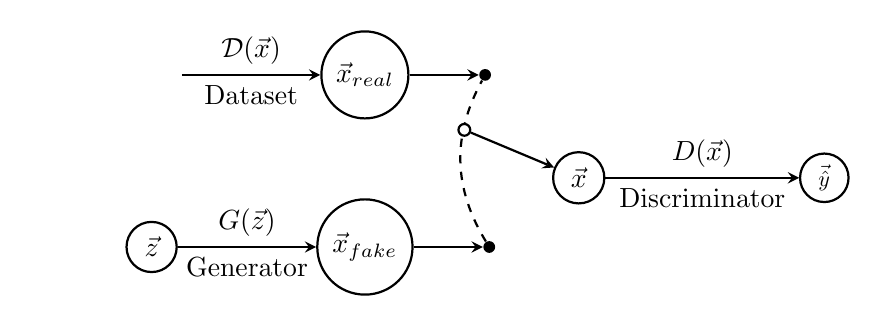
\begin{tikzpicture}
	\node[circle, draw, thick] (z) {$\vec{z}$};
	\node[circle, draw, thick, right=5em of z] (x) {$\vec{x}_{fake}$};
	\draw[-stealth, thick] (z) -- node[above] {$G(\vec{z})$} node[below] {Generator} (x);
	\node[left=of z] (i) {};
	\node[above=of x, circle, draw, thick] (xt) {$\vec{x}_{real}$};
	\node[left=5em of xt] (it) {};
	\draw[-stealth, thick] (it) -- node[above] {$\mathcal{D}(\vec{x})$} node[below] {Dataset} (xt);
	\node[circle, draw, thick, right=5em of x, yshift=2.5em] (D) {$\vec{x}$};
    \node[circle, scale=0.80, draw, thick, right=7em of D] (out) {$\vec{\hat{y}}$};
	\draw[-stealth, thick] (D) -- node[above] {$D(\vec{x})$} node[below] {Discriminator} (out);
	\node[right=2.5em of x, circle, fill, inner sep=0.15em] (pt1) {};
	\node[right=2.5em of xt, circle, fill, inner sep=0.15em] (pt2) {};
	\draw[dashed, thick] (pt1) edge[bend left] (pt2);
	\node[circle, draw, thick, fill=white, inner sep=0.15em] at ([xshift=-0.9em, yshift=4em]pt1.north) (pt3) {};
	\draw[-stealth, thick] (x) -- (pt1);
	\draw[-stealth, thick] (xt) -- (pt2);
	\draw[-stealth, thick] (pt3) -- (D);
\end{tikzpicture}
\par}

\subsection{PCG Classifier (GAN)}
The PCG arrhythmia detection algorithm is a sequence-to-sequence Generative Adversarial Network, with the architecture that contains a Generator (\($G$\)) and a Discriminator (\($D$\)). The function of a Generator is to generate data such that, the Discriminator will classify the generated data as real, while the Discriminator aims to classify the generated data as fake. Hence, the Generator requires a series of noise signals \($z_{i} \sim N\left (\mu,\sigma^{2}\right)$\); such that \($\mu=0$\) and \($\sigma=1$\). Thus, \($\overrightarrow{z}\in\{-1,1\}$\) where every element of \($z$\) is between \($-1$\) and \($1$\), with a fixed length \($z_{100}$\). The Generator then outputs \($\overrightarrow{x}_{fake}=[x_{1},...x_{n}]$\) biased on \($\overrightarrow{z}$\). Conversely, the Discriminator takes inputs \($ \overrightarrow{x}=[x_{1},...x_{n}]$\) as features from a dataset, $\mathcal{D}$, and calculates the outputs \($\overrightarrow{\hat{y}}= [\hat{y_{1}},...\hat{y_{c}}]$\) based on latent features extracted from \($ \overrightarrow{x}$\), where \($\hat{y_{i}}-1$\) represents each class in the dataset. Given \($\left |\overrightarrow{x}_{fake}\right |\sim\left |\overrightarrow{x}\right |$\), meaning the Generator output, \($\overrightarrow{x}_{fake}$\) is similar in structure and cardinality with the input of the Discriminator, \($\overrightarrow{x}$\).

\subsection{PCG Constructor}
Note: Ideally I would use a GAN, LSTM, but if I don't have enough time I can use the research done \href{https://www.sciencedirect.com/science/article/abs/pii/S1746809413000037}{here}. All add more inf oration once classifier accuracy reaches about 80/%. 

\section{Database}
\subsection{PCG Databases}
Although PCG signals are analyzed less often than ECG signals, these signals are rather analyzed in real-time by physicians and healthcare workers. Preliminary studies done on PCG segmentation and classification primarily used private datasets. Hence, there existed no publicly available datasets until recently. Since then, many public datasets have been developed aiding researchers in their studies and creating open benchmarks for researchers to use in comparing similar findings. However, these datasets are still limited by the number of classes that are collected, when compared to ECG datasets.

Currently, only three major supervised PCG datasets exist: PhysioNet Classification of Heart Sound Recording Challenge dataset [source], PASCAL Heart Sound Challenge dataset [source], and the Heart Sound and Murmur Library [source].  These datasets are all anonymized and de-identified for the safety of their subjects, and thus includes no personal information such as name, income, age, etc.

The PhysioNet Classification of Heart Sound Recording Challenge dataset was produced as a part of the 2016 PhyisoNet Computing in Cardiology Challenge. The heart sounds were collected from both clinical and non-clinical environments (in-home visits). The challenge focused on creating an accurate dataset of normal and abnormal heart sound recordings, especially in real-world (extremely noisy and low signal quality) scenarios. These recordings were sourced from nine independent databases and in total, contain 4,593 heart sound recordings from 1072 subjects, lasting from 5-120 seconds. Of which, 409 recordings that were collected from 121 patients contain one PCG lead and one simultaneously recorded ECG. Though, all recordings were resampled to 2,000 Hz using an anti-alias filter. Furthermore, the dataset is comprised of 3 classes: normal, abnormal, and unsure (this is due to poor recording quality), and have the following proportion respectively: 77.1\%, 12,0\%, 10.9\%  \href{https://www.ncbi.nlm.nih.gov/pmc/articles/PMC7199391/pdf/nihms-1005138.pdf}{[source]}. 

The PASCAL Classifying Heart Sounds Challenge dataset was released to the general public in 2011. The challenge consisted of two sub-challenges: heart sound segmentation, and heart sounds classification; these sub-challenges corresponded with dataset A, and dataset B respectively. Both datasets have recordings of of varying lengths, between 1 second and 30 seconds. Dataset A was collected via the iSethoscope Pro iPhone app, and contained 176 heart sound recording. 124 of which are divided into four classes: Normal (31 recordings), Murmur (34 recordings), Extra heart sound (19 recordings), and Artifact (40 recordings); the rest of the records are unlabeled for testing purposes. Dataset B was collected using a DigiScope (a digital stethoscope), and included 656 heart sounds. All expect 370 were separated into three classes: Normal (320 recordings), Murmur (95 recordings), and Extra-systole (46 recordings). Both datasets A and B vary in sound recordings  between lengths of 1 second and 30 second \href{http://www.peterjbentley.com/heartchallenge/}{[source]}.

The Heart sound and Murmur Library provided by the University of Michigan Health Systems, is a dataset that contains Normal, Mitral Valve Prolapse, Acute Mitral Regurgitation, Left Ventricular Hypertrophy, Dilated Cardiomyopathy with Mitral Regurgitation, Mitral Stenosis, Aortic Regurgitation, Combined Aortic Stenosis and Regurgitation, Arterial Septal Defect, and Pulmonary Valve Stenosis at the Apex, Aortic, and Pulmonic Area \href{http://www.med.umich.edu/lrc/psb_open/html/repo/primer_heartsound/primer_heartsound.html}{[source]}.

\subsection{ECG Databases}
More than 300 million ECG recordings are analyzed yearly \href{https://pubmed.ncbi.nlm.nih.gov/10516892/}{[source]}, and thus create an exceptional tool for arrhythmia classification. Coupled with the recent surge in research interest in 2015, many massive publicly available datasets have been published, notable by PhysioNet - the moniker of the Research Resource for Complex Physiologic Signals \href{https://physionet.org/about/}{[source]}. Numerous, datasets ECG exit, however, many are limited to few classes (Normal and Abnormal). At present, three public datasets exist that have more than 4 classes: AF Classification Challenge 2017 \href{https://physionet.org/content/challenge-2017/1.0.0/)}{[source]}, PTB Diagnostic ECG \href{https://www.physionet.org/content/ptbdb/1.0.0/)}{[source]}, and PTB-XL dataset \href{https://physionet.org/content/ptb-xl/1.0.1/)}{[source]}. Additionally, iRhythm Technologies have developed a semi-public dataset, that is available upon request, that contains 12 classes \href{https://www.nature.com/articles/s41591-018-0268-3}{[source]}.

The PTB-XL is the largest publicly available dataset for ECGs and contains 21,837 clinical 12-lead ECG recordings from 18,885 patients of 10 second length. Theses recordings are separated into 5 super-classes: Normal, Myocardial Infraction, Hypertrophy, ST/T-Change, and Conduction Disturbance. These super-classes are further split into 71 sub-classes that range from AV Block to Posterior Myocardial Infraction. The raw signal data was downsampled to 100 Hz and annotated by up to two cardiologists, who assigned potentially multiple ECG statements to each record.
\href{https://physionet.org/content/ptb-xl/1.0.1/}{[source]}.

iRhythm Technologies developed a large, 12 classes ECG dataset using raw single-lead ECG inputs. The 12 classes include Atrial fibrillation and flutter, AVB, Bigeminy, EAR, IVR, Junctional rhythm, Noise, Sinus rhythm, SVT, Trigeminy, Ventricular tachycardia, and Wenckebach. The dataset consists of 91,232 ECG recordings from 53,549 patients. This training dataset is available upon request under license from iRhythm Technologies, Inc. The test dataset, which is publicity available, contains 328 records collected from 328 unique patients, split between 6 classes. Both datasets were recorded using a Zio monitor, which monitors the heart through a single-lead sensor at  200 Hz. The annotation was done by a consensus committee of expert cardiologists \href{https://www.nature.com/articles/s41591-018-0268-3}{[source]}.

The PhysioNet AF Classification database, presented in 2017 for the Computing in Cardiology Challenge, contains 8,528 ECG recordings, divided into 4 classes: Normal (5154 recordings), Atrial Fibrillation (771 recordings), Other arrhythmias (2557 recordings), and Noisy (46 recordings). The single-lead recordings last from 9 - 61 seconds, with an a mean of 32.5 seconds and a standard deviation of 10.9 seconds. The ECG recordings were sampled to 300 Hz and provided in MATLAB V4 WFDB-compliant format \href{https://physionet.org/content/challenge-2017/1.0.0/}{[source]}.

\section{Methodology}
Note: I plant to discuss the following: 
- Model
- Pre-processing
    - Asses signal quailty
    - Filter out baseline changes (low/high band pass filter)
    - Time/Frequency/Time-Frequency
- Segmentation
    - Delineate the start of each phase (S1, Systole, S2, Diastole, ect)
- Normilzation
- Standardization
- Data Augmentation
- Data Transformation
- Classification
- Training/Validation/Testing
- Metrics

\subsection{Approach}
The training phase involves 3 stages: AE training, AE+GAN training, and GAN fine-tuning. During training phases, all datasets will follow the following split: 70\% - training, 15\% - validation, 15\% - testing; this cross-validation step validates that both models are not overfitting during the training phase. The first stage involves training the AE with a supervised dataset of ECG and PCG signals (Liu et al, 2016). The second stage involves training both the AE and the GAN with a supervised dataset of arrhythmias within ECGs (Goldberger et al., 2017). During the training process, the AE model will be frozen (the weights and biases of the AE model won't be trained) as this process is already done in the preceding stage. The last stage is fine-tuning the GAN  on a binary supervised dataset of PCG signals (Normal vs Abnormal). This validates the model's metrics in the previous step.  
\begin{center}
    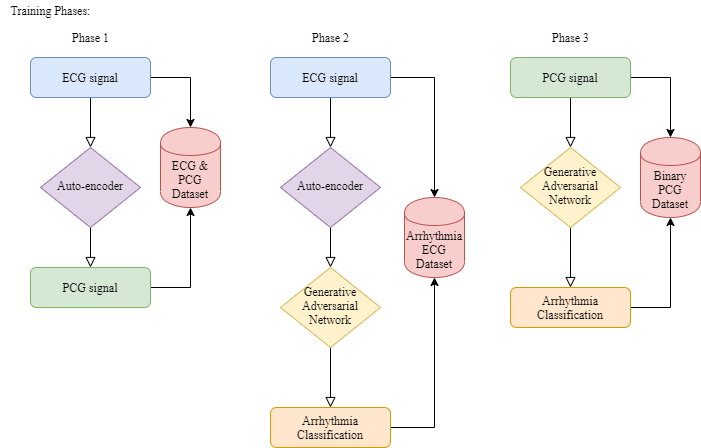
\includegraphics[scale=0.70]{training-digram}
\end{center}

\subsection{Goals}
While testing and training, the model will be validated against with metrics such as recall, precision, accuracy, loss, FBeta, F1 score, and ROC/AUC score. These tests will ensure that the model is accurately predicting the classes, and identifying important features within the datasets. Each step in the training phase will represent a milestone and an accuracy of 97\% will mark the completion criteria.

\subsection{Risks}
\paragraph{Overfitting:}
One of the largest problems in Deep Learning overall, which possesses a threat to our model is overfitting. Overfitting typically happens when the model metrics of the training and validation set diverge. This suggests that the model is not generalizing, but rather memorizing the training dataset. To combat overfitting, researchers typically implement data argumentation techniques to reinforce important features in a dataset. 

\paragraph{Domain Shift:}
A domain shift occurs when a source dataset performs well but on a different dataset distribution, the performance drastically decreases. Typically, domain adaptation is often used to improve performance on target datasets. This is done by training the model itself on multiple datasets to improve the model's capacity to generalize.

\paragraph{Traning Time:}
With large multi-model architectures, it becomes tough to train models on a single GPU. This can happen for a number of reasons, but the main reason is because the model takes up too much memory of the GPU. Generally, parallel processing is used to split tasks and assign them to different GPUs. For instance, the AE model will run on a single GPU, while the GAN will run on another GPU.

\subsection{Project Budget}
\begin{tabular}{lllll}
                & Price per Hour & Hours      & Cost   &  \\
NVIDIA A100 GPU & \$3.10         & 225        & 697.50 &  \\
                &                & Total Cost & 697.50 &  \\
                &                &            &        & 
\end{tabular}

\section*{Acknowledgement}
I thank Professor Lifang He of Leigh University for helpful guidance and feedback on the experiments and references.

\bibliographystyle{unsrt}  
%\bibliography{references}  %%% Remove comment to use the external .bib file (using bibtex).
%%% and comment out the ``thebibliography'' section.


%%% Comment out this section when you \bibliography{references} is enabled.
\begin{thebibliography}{1}
\end{thebibliography}


\end{document}
